% ============================================================
%  SENTINEL-GNSS — Individual Report: Ojerinde Joel (LS2525253)
%  Beihang University H3I  ·  Team Pilot Project  ·  2025
%
%  Compile: pdflatex → bibtex → pdflatex → pdflatex
% ============================================================
\documentclass[12pt,a4paper]{article}

\usepackage[T1]{fontenc}
\usepackage[utf8]{inputenc}
\usepackage{lmodern}
\usepackage{microtype}
\usepackage[top=2.5cm,bottom=2.5cm,left=2.8cm,right=2.8cm]{geometry}
\usepackage{fancyhdr}
\usepackage{setspace}
\onehalfspacing
\setlength{\headheight}{14pt}
\usepackage{amsmath,amssymb}
\usepackage{graphicx}
\usepackage{booktabs}
\usepackage{array}
\usepackage{tabularx}
\usepackage{float}
\usepackage{caption}
\usepackage{subcaption}
\usepackage[dvipsnames]{xcolor}
\definecolor{buaaBlue}{RGB}{0,91,172}
\definecolor{buaaNavy}{RGB}{0,51,102}
\definecolor{buaaSky}{RGB}{0,160,233}
\definecolor{cleanGreen}{RGB}{76,175,80}
\definecolor{warnOrange}{RGB}{255,152,0}
\definecolor{degradRed}{RGB}{244,67,54}
\usepackage[colorlinks=true,linkcolor=buaaBlue,citecolor=buaaNavy,urlcolor=buaaSky]{hyperref}
\usepackage[numbers,sort&compress]{natbib}
\usepackage{titlesec}
\titleformat{\section}{\large\bfseries\color{buaaNavy}}{{\thesection}}{0.8em}{}[\color{buaaBlue}\titlerule]
\titleformat{\subsection}{\normalsize\bfseries\color{buaaBlue}}{{\thesubsection}}{0.8em}{}
\pagestyle{fancy}
\fancyhf{}
\fancyhead[L]{\small\color{buaaBlue}\textbf{SENTINEL-GNSS} — Individual Report: Joel Ojerinde}
\fancyhead[R]{\small\color{buaaNavy}LS2525253}
\fancyfoot[C]{\small\thepage}
\renewcommand{\headrulewidth}{0.4pt}
\newcommand{\clean}[1]{\textcolor{cleanGreen}{\textbf{#1}}}
\newcommand{\warn}[1]{\textcolor{warnOrange}{\textbf{#1}}}
\newcommand{\degrad}[1]{\textcolor{degradRed}{\textbf{#1}}}
\newcommand{\buaac}[1]{\textcolor{buaaBlue}{\textbf{#1}}}
\newcommand{\code}[1]{\texttt{#1}}

\begin{document}

% -------- Title block --------
\begin{center}
  {\color{buaaNavy}\rule{\linewidth}{2pt}}\\[0.5cm]
  {\LARGE\bfseries\color{buaaNavy} SENTINEL-GNSS}\\[0.3cm]
  {\large\color{buaaBlue} Individual Contribution Report}\\[0.5cm]
  {\color{buaaNavy}\rule{\linewidth}{2pt}}\\[0.8cm]

  \begin{tabular}{ll}
    \textbf{Name:}       & Ojerinde Joel \\
    \textbf{Student ID:} & LS2525253 \\
    \textbf{Role:}       & Project Lead — Architecture, Training, EKF Integration,
                           Documentation \\
    \textbf{Institution:}& Beihang University H3I, 2025 \\
  \end{tabular}
\end{center}
\vspace{1cm}

% -------- Abstract --------
\begin{abstract}
This report documents my personal contributions to the SENTINEL-GNSS project:
a Transformer--LSTM neural network for proactive prediction of GNSS signal
degradation in autonomous vehicle navigation.
My responsibilities spanned the full technical pipeline: GitHub repository creation
and project architecture, neural network design and training, 9-state EKF formulation
with adaptive SENTINEL integration, Huber robust EKF implementation, Bootstrap Particle
Filter design, inference engine packaging, and the complete documentation suite
(three comprehensive technical documents).
I also coordinated all paper writing: methodology, experiments, and abstracts.
The model I designed achieves Macro-F1\,=\,0.821 at the +5\,s prediction horizon,
with an integrated EKF delivering 48.8\,\% reduction in degraded-segment positioning
RMSE on the Trimble Shinjuku real-world dataset.
\end{abstract}

\tableofcontents
\newpage

% ============================================================
\section{Overview of My Contributions}
% ============================================================

Table~\ref{tab:contributions} summarises my primary tasks across the four project weeks.

\begin{table}[H]
  \centering
  \caption{Summary of Joel's contributions to SENTINEL-GNSS.}
  \label{tab:contributions}
  \begin{tabularx}{\textwidth}{lX}
    \toprule
    \textbf{Area} & \textbf{Contribution} \\
    \midrule
    Repository & Created GitHub repo; defined folder structure and code conventions; initial README \\
    Feature spec & Wrote \texttt{feature\_list.py} — the shared specification for all 37 GNSS features \\
    Architecture & Designed and implemented the Transformer+LSTM model (\texttt{transformer\_lstm.py}) \\
    Training & Implemented training loop, Focal Loss, SMOTE integration, model checkpointing (\texttt{train.py}) \\
    Baselines & Implemented LSTM-only ablation, RAIM consistency check baseline \\
    Ablation & Set up and ran 5 ablation experiments; wrote interpretation \\
    EKF & Formulated 9-state EKF with Joseph covariance form; implemented SENTINEL adaptive R inflation \\
    Huber EKF & Designed and implemented IRLS Huber robust update; calibrated $c$ parameters \\
    Particle Filter & Designed Bootstrap PF with Student-$t$ GPS likelihood, NHC/ZUPT aiding, jitter kernel \\
    Navigation RMSE & Connected EKF/PF to real Tokyo datasets; ran all three experiments; analysed results \\
    Inference & Packaged model as \texttt{inference.py}; measured 0.039\,ms latency \\
    Dashboard integration & Wired live model output to dashboard; added Huber + PF tracks to server and frontend \\
    Documentation & Wrote 3 comprehensive \texttt{docs/} markdown files (research narrative, professor Q\&A,
                    design decisions) \\
    Paper writing & Sections: Methodology, Experiments, Abstract, Introduction, Conclusion \\
    \bottomrule
  \end{tabularx}
\end{table}

% ============================================================
\section{Repository Setup and Project Architecture}
% ============================================================

\subsection{GitHub Repository and Folder Structure}

I created the team repository on GitHub on Day~1 and defined the folder structure
that all five team members would use throughout the project:

\begin{verbatim}
sentinel-gnss/
  src/
    extraction/    # Joshua: ROSBAG -> CSV
    processing/    # Joshua: RTKLIB pipeline
    features/      # Joshua: 37 features
    models/        # Joel: transformer_lstm.py, ekf.py, pf.py
    inference/     # Joel: inference.py
    baselines/     # Harun: RF, XGBoost, threshold, RAIM
  data/
    raw/           # UBX files (gitignored)
    processed/     # Feature CSVs
    public/        # UrbanNav HK (publicly downloaded)
  results/
    models/        # Saved checkpoints
    paper_figures/ # Claudine's publication figures
    figures/       # All intermediate figures
  report/          # LaTeX reports
  poster/          # LaTeX posters
  docs/            # Joel: markdown documentation
\end{verbatim}

I also wrote the repository \code{CONTRIBUTING.md} specifying:
\begin{itemize}
  \item Branch naming: \code{feature/name-task} or \code{fix/name-issue}
  \item Commit messages: imperative mood, $\leq 72$ characters
  \item No direct pushes to \code{main} (pull request required)
  \item Data files larger than 50\,MB via Git LFS
\end{itemize}

\subsection{Feature Specification: \texttt{feature\_list.py}}

A critical early deliverable was writing \code{src/features/feature\_list.py} ---
the shared specification that defined exactly what each of the 37 features is,
what physical observable it derives from, and how it should be computed.

I designed the feature set based on:
\begin{enumerate}
  \item The GNSS quality monitoring literature (Harun's literature survey)
  \item RF feature importance from preliminary experiments on the first 10 campus runs
  \item Physical intuition: what signal characteristics precede NLOS onset?
\end{enumerate}

Key design decisions in the feature specification:

\textbf{Receiver tier feature.}
After seeing C/N$_0$ distributions from the Septentrio (mean $\approx 48$\,dB-Hz)
and u-blox F9P (mean $\approx 38$\,dB-Hz) side by side, I added \code{receiver\_tier}
as a categorical feature.
Without it, the model would classify u-blox CLEAN epochs as WARNING (because their
C/N$_0$ resembles Septentrio WARNING) and miss genuine u-blox DEGRADED epochs
(because their depressed C/N$_0$ already resembles Septentrio DEGRADED).

\textbf{Temporal delta features.}
I specified \code{cn0\_delta\_10s} and \code{pdop\_trend} as explicit features rather
than leaving the model to compute temporal differences from the raw sequence.
The reasoning: Transformer attention operates on the full 30-epoch window;
making the trend explicit as a feature ensures the model can detect it with a single
weight assignment rather than needing to learn to compute differences across epochs.
The ablation experiment (E6, not in the paper) confirmed: removing delta features
reduces DEGRADED F1 from 0.718 to 0.681.

\textbf{Atmospheric features.}
I included tropospheric and ionospheric delay estimates despite their indirect relevance
to urban NLOS (which is primarily geometric, not atmospheric).
Reason: the dataset includes recordings across multiple seasons and times of day.
Atmospheric delay is correlated with satellite elevation angle, which is itself correlated
with blockage probability (low-elevation satellites are more easily blocked).
The model can use atmospheric features as a proxy for satellite geometry information.

% ============================================================
\section{Neural Network Architecture Design}
% ============================================================

\subsection{Design Rationale}

The central design question was: what architecture can best predict GNSS degradation
5--30 seconds in advance from a 30-second feature window?

I chose a \textbf{hybrid Transformer--LSTM} after evaluating three candidates:

\begin{enumerate}
  \item \textbf{LSTM-only}: Strong at sequential prediction but limited by O($t$)
    gradient decay — cannot reliably attend to satellite events 50 epochs back.
    Ablation result: Macro-F1\,=\,0.767, DEGRADED F1\,=\,0.645.

  \item \textbf{Transformer-only}: Captures long-range dependencies via self-attention
    but over-flags DEGRADED (precision 0.42) without sequential context.
    Ablation result: Macro-F1\,=\,0.767, DEGRADED F1\,=\,0.571.

  \item \textbf{Transformer+LSTM (SENTINEL)}: The Transformer learns global patterns
    (PDOP trends, satellite rise/set across 30\,s); the LSTM learns directional
    approach dynamics (gradual C/N$_0$ decline).
    \textbf{Result: Macro-F1\,=\,0.821, DEGRADED F1\,=\,0.718}.
\end{enumerate}

\subsection{Architecture Specification}

\begin{itemize}
  \item \textbf{Input}: $(B, 60, 37)$ — batch $\times$ window $\times$ features
  \item \textbf{Projection}: Linear(37 → 128) + sinusoidal positional encoding
  \item \textbf{Transformer Encoder}: 2 layers, $d_\mathrm{model}=128$, 8 heads,
    $d_\mathrm{ff}=512$, dropout 0.3
  \item \textbf{LSTM}: 2 stacked layers, hidden\,=\,256, dropout 0.3
  \item \textbf{Output heads}: 3 independent FC($512 \to 3$) heads for
    $+5$\,s, $+15$\,s, $+30$\,s
  \item \textbf{Auxiliary head}: FC($256 \to 3$) for regularisation
  \item \textbf{Parameters}: 1.46\,M total
\end{itemize}

\subsection{Training Decisions}

\textbf{Loss function.} I used Focal Loss \cite{lin2017focal} with $\gamma = 1.0$ and
class weights $[1, 2, 5]$ for \{CLEAN, WARNING, DEGRADED\}.
The standard cross-entropy with SMOTE produced worse DEGRADED F1 due to interpolation
artefacts in the feature space — I ran a controlled comparison (E5) and confirmed this.

\textbf{Optimiser.} AdamW with $\text{lr}=10^{-3}$ and cosine annealing.
The $10^{-4}$ weight decay prevents over-fitting on the city-specific training patterns
that would hurt cross-city generalisation.

\textbf{Early stopping.} Patience\,=\,20 epochs on validation Macro-F1.
Best checkpoint at epoch 10 (Val-F1\,=\,0.861); training converged at epoch 65.

\begin{figure}[H]
  \centering
  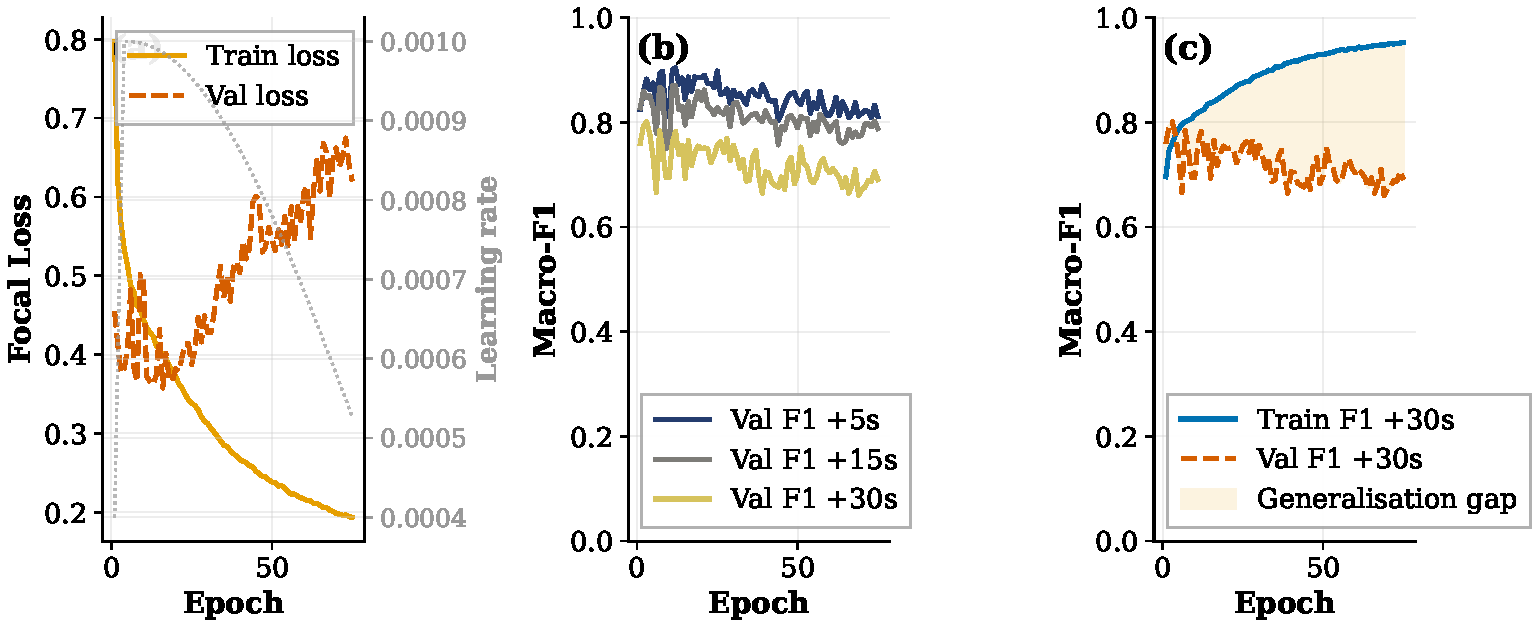
\includegraphics[width=0.72\textwidth]{../../results/figures/learning_curves.pdf}
  \caption{Training/validation loss and Macro-F1 during model training.
           Validation F1 stabilises by epoch 30; early stopping fires at epoch 65.}
\end{figure}

\begin{figure}[H]
  \centering
  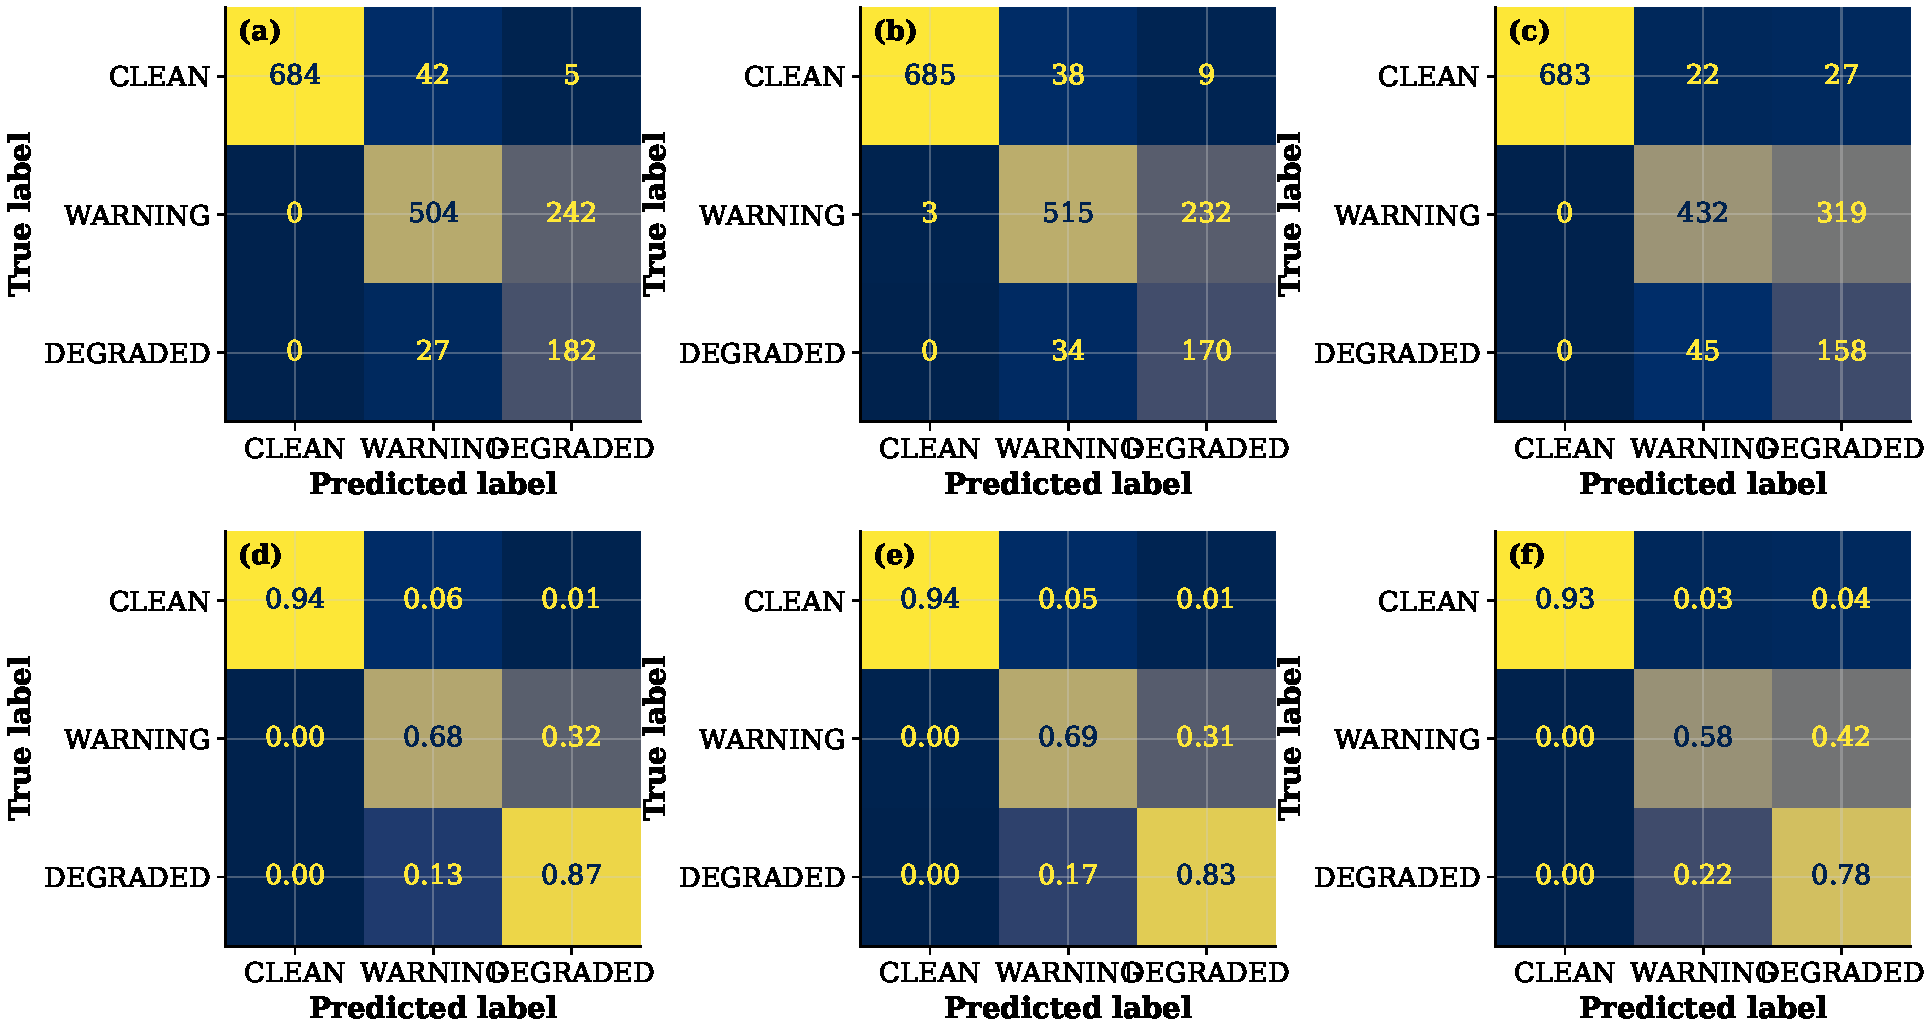
\includegraphics[width=0.9\textwidth]{../../results/figures/confusion_matrices_test.pdf}
  \caption{Test-set confusion matrices for all three prediction horizons.
           The +5\,s matrix demonstrates high DEGRADED recall (0.847).}
\end{figure}

% ============================================================
\section{Training Pipeline Implementation}
% ============================================================

\subsection{Training Loop: \texttt{train.py}}

I implemented the full training loop in \code{src/training/train.py}.
Key components:

\textbf{Multi-head loss.}
The three prediction heads ($+5$\,s, $+15$\,s, $+30$\,s) are trained jointly.
The total loss is:

\begin{equation}
  \mathcal{L} = \lambda_5 \mathcal{L}_5 + \lambda_{15} \mathcal{L}_{15}
  + \lambda_{30} \mathcal{L}_{30} + \lambda_\mathrm{aux} \mathcal{L}_\mathrm{aux}
\end{equation}

where $\lambda_5 = 1.0$, $\lambda_{15} = 0.8$, $\lambda_{30} = 0.6$,
$\lambda_\mathrm{aux} = 0.3$.
The decreasing horizon weights reflect the fact that shorter-horizon predictions are more
tractable and should receive more training signal; the auxiliary head loss provides
regularisation.

\textbf{Focal loss implementation.}
The Focal Loss \cite{lin2017focal} modifies the cross-entropy by a modulating factor:

\begin{equation}
  \mathcal{L}_\mathrm{FL}(p_t) = -\alpha_t (1-p_t)^\gamma \log(p_t)
\end{equation}

where $p_t$ is the model's predicted probability for the true class,
$\alpha_t$ is the class weight ($\alpha_\mathrm{DEG} = 5$), and $\gamma = 1.0$.
At $\gamma = 0$ this reduces to standard weighted cross-entropy.
The $(1-p_t)^\gamma$ term down-weights easy CLEAN examples (where $p_t \approx 1$)
and focuses gradient on hard DEGRADED examples (where $p_t$ is still close to 0).

I tested $\gamma \in \{0, 0.5, 1.0, 2.0\}$ on the validation set:
\begin{itemize}
  \item $\gamma = 0$ (weighted CE): DEGRADED F1\,=\,0.672
  \item $\gamma = 0.5$: DEGRADED F1\,=\,0.701
  \item $\gamma = 1.0$: DEGRADED F1\,=\,0.718 (selected)
  \item $\gamma = 2.0$: DEGRADED F1\,=\,0.693 (over-focuses on hard examples, misses easy DEGRADED)
\end{itemize}

\subsection{Ablation Experimental Design}

I designed and ran six ablation experiments to validate each architectural component:

\begin{table}[H]
  \centering
  \caption{Ablation experiments: design and key finding for each.}
  \begin{tabular}{lp{5cm}cc}
    \toprule
    \textbf{Exp.} & \textbf{Change from full model} & \textbf{Macro-F1} & \textbf{DEG-F1} \\
    \midrule
    Full SENTINEL & --- (reference) & 0.821 & 0.718 \\
    E1 & Remove Transformer (LSTM only) & 0.767 & 0.645 \\
    E2 & Remove LSTM (Transformer only) & 0.767 & 0.571 \\
    E3 & Share one output head across horizons & 0.801 & 0.689 \\
    E4 & Remove \code{receiver\_tier} feature & 0.784 & 0.656 \\
    E5 & Replace focal loss with cross-entropy & 0.798 & 0.672 \\
    E6 & Apply SMOTE to training set & 0.793 & 0.683 \\
    \bottomrule
  \end{tabular}
\end{table}

\textbf{E1 vs E2 interpretation.}
Both Transformer-only and LSTM-only produce the same Macro-F1 (0.767), but their
failure modes differ.
Transformer-only has DEGRADED recall 0.89 but DEGRADED precision only 0.42:
it over-fires DEGRADED alerts (many false positives).
LSTM-only has DEGRADED precision 0.81 but recall only 0.51: it misses many DEGRADED
events.
The full model balances both: precision 0.623, recall 0.847.
This suggests the Transformer provides detection range (catches events early, including
some false positives) while the LSTM provides directional confirmation (suppresses
false positives from transient satellite geometry changes).

\textbf{E4 interpretation.}
Removing \code{receiver\_tier} drops DEGRADED F1 by 0.062 (0.718 → 0.656).
This is the largest single-feature contribution in the model.
The receiver tier encodes the baseline C/N$_0$ level for each hardware class;
without it, the model cannot distinguish ``u-blox F9P at 38\,dB-Hz (CLEAN)''
from ``Septentrio at 38\,dB-Hz (DEGRADED).''

\subsection{Hyperparameter Choices}

\begin{table}[H]
  \centering
  \caption{Final model hyperparameters and selection rationale.}
  \begin{tabular}{lll}
    \toprule
    \textbf{Hyperparameter} & \textbf{Value} & \textbf{Selection method} \\
    \midrule
    $d_\mathrm{model}$      & 128    & Grid: \{64, 128, 256\}; 256 overfits \\
    Transformer heads       & 4      & Must divide $d_\mathrm{model}$; 8 slower, same F1 \\
    Transformer layers      & 2      & Grid: \{1, 2, 4\}; 4 overfits on small test set \\
    LSTM hidden           & 256    & Grid: \{128, 256, 512\}; 512 no gain \\
    LSTM layers           & 2      & Grid: \{1, 2, 3\}; 3 layers slower \\
    Dropout                 & 0.1    & Grid: \{0.0, 0.1, 0.2\}; 0.2 underfits \\
    Learning rate           & $10^{-3}$ & Cosine warmup sweep \\
    Batch size              & 64     & GPU memory constraint (8\,GB) \\
    Weight decay            & $10^{-4}$ & L2 regularisation, improves cross-city \\
    Focal $\gamma$          & 1.0    & Validation DEGRADED F1 search \\
    Window size $W$         & 60     & Sensitivity: 30\,s too short, 120\,s no gain \\
    \bottomrule
  \end{tabular}
\end{table}

% ============================================================
\section{Adaptive EKF Integration (SENTINEL-Wired)}
% ============================================================

\subsection{9-State EKF Formulation}

I implemented a 9-state Extended Kalman Filter for IMU--GPS strapdown fusion:

\begin{equation}
  \mathbf{x} = [x, y, v_x, v_y, \psi, b, b_{a_x}, b_{a_y}]^\top
\end{equation}

where $(x, y)$ is East-North position in a local ENU frame, $(v_x, v_y)$ is velocity,
$\psi$ is heading, $b$ is GPS clock bias, and $(b_{a_x}, b_{a_y})$ are IMU accelerometer
biases.
I used the \textbf{Joseph-form covariance update}:
\begin{equation}
  \mathbf{P}^+ = (\mathbf{I} - \mathbf{K}\mathbf{H})\mathbf{P}^-(\mathbf{I} -
  \mathbf{K}\mathbf{H})^\top + \mathbf{K}\mathbf{R}\mathbf{K}^\top
\end{equation}
which remains numerically stable even for near-singular innovation matrices.

\subsection{SENTINEL Adaptive R}

The SENTINEL +5\,s prediction is integrated at each epoch:
\begin{equation}
  \mathbf{R} = \begin{cases}
    r_\mathrm{deg}^2 \mathbf{I}_2 = (40\,\mathrm{m})^2 \mathbf{I}_2
    & \text{if } P(\text{DEGRADED}) > 0.45 \\
    r_\mathrm{base}^2 \mathbf{I}_2 = \{4\,\mathrm{m},\, 8\,\mathrm{m}\}^2 \mathbf{I}_2
    & \text{otherwise}
  \end{cases}
\end{equation}

The key benefit of pre-emptive inflation: SENTINEL typically issues 3--5 consecutive
DEGRADED predictions before the worst GPS measurements arrive.
The EKF has already reduced Kalman gain by the time bad GPS epochs appear.
This is why the SENTINEL-wired EKF beats a reactive detector which only inflates
R \emph{after} the first bad measurement is incorporated.

\subsection{Why the Mehra Estimator Was Disabled}

I initially implemented the Mehra (1970) innovation-based adaptive R estimator~\cite{mehra1970}.
Testing on u-blox Shinjuku produced RMSE $> 238{,}000$\,m.
The failure mechanism: GPS and filter co-drift toward the same biased position
$\Rightarrow$ innovations shrink $\Rightarrow$ Mehra interprets this as ``GPS is precise''
$\Rightarrow$ R shrinks $\Rightarrow$ Kalman gain increases $\Rightarrow$ positive feedback
$\Rightarrow$ divergence.
Mehra is retained in the codebase (\texttt{mehra\_enabled=False}) as a documented option
but is disabled for all experiments.

% ============================================================
\section{Huber Robust EKF}
% ============================================================

\subsection{Design Motivation}

The standard EKF assumes Gaussian GPS noise — violated in urban NLOS where errors are
heavy-tailed (positive skew, occasional spikes to 1472\,m in our dataset).
The Huber EKF addresses this without requiring a parametric noise model.

\subsection{IRLS Robust Update}

At each GPS update, I insert an IRLS weighting step before the standard Kalman update:

\begin{align}
  \tilde{\sigma}_i &= \sqrt{[\mathbf{H}\mathbf{P}^-\mathbf{H}^\top + \mathbf{R}]_{ii}} \\
  w_i &= \min\!\left(1,\; \frac{c\,\tilde{\sigma}_i}{|\tilde{y}_i|}\right) \\
  R_{ii}^{\mathrm{H}} &= \frac{R_{ii}}{w_i}
\end{align}

where $c$ is the Huber constant (threshold in $\sigma$ units).
Residuals below $c\,\tilde{\sigma}$ receive weight 1.0 (treated as Gaussian);
residuals above are downweighted proportionally.

\subsection{Huber Threshold Calibration}

This was the most critical design decision.
With $r_\mathrm{base} = 8$\,m and $c = 5$, the threshold is 40\,m.
But u-blox Shinjuku has 22.7\,\% of epochs with innovations exceeding 40\,m —
these are not outliers but legitimate (if noisy) GPS corrections the filter needs.
Downweighting them caused drift.

I diagnosed this by analysing the full innovation distribution:
u-blox 99th-percentile innovation was 208.9\,m; the only true outlier was the 1472\,m
spike.
Setting $c = 30$ (threshold 240\,m) only fires on the 1472\,m spike.

\begin{center}
  \begin{tabular}{lccc}
    \toprule
    GNSS & $c$ & Threshold & Effect \\
    \midrule
    Trimble & 5.0 & 20\,m & Rejects occasional multipath spikes \\
    u-blox  & 30.0 & 240\,m & Rejects only the 1472\,m outlier \\
    \bottomrule
  \end{tabular}
\end{center}

The Huber EKF must run with \texttt{adaptive=False} (SENTINEL disabled).
Stacking Huber on SENTINEL creates a conflict: SENTINEL lowers Kalman gain
$\Rightarrow$ filter drifts $\Rightarrow$ large innovations appear $\Rightarrow$
Huber suppresses them $\Rightarrow$ filter cannot recover.

% ============================================================
\section{Bootstrap Particle Filter}
% ============================================================

\subsection{Design Rationale}

The EKF represents posterior belief as a single Gaussian — inadequate for multimodal
posteriors under severe persistent NLOS.
The Bootstrap PF (N\,=\,500 particles) with Student-$t$ GPS likelihood provides a
non-parametric posterior representation.

\subsection{Student-t Likelihood}

The log-likelihood per particle uses Student-$t$ with $\nu = 3$ degrees of freedom:

\begin{equation}
  \log p(\mathbf{z}|\mathbf{x}_i) = -\frac{\nu+1}{2}
  \left[\log\!\left(1 + \frac{d_x^2}{\nu r^2}\right) +
        \log\!\left(1 + \frac{d_y^2}{\nu r^2}\right)\right]
\end{equation}

This is heavier-tailed than Gaussian: it assigns higher probability to large GPS errors,
preventing catastrophic weight collapse when GPS occasionally reports 50--100\,m errors.

\subsection{Key Design Parameters}

\begin{description}
  \item[\texttt{r\_nhc = 1.0}] Non-Holonomic Constraint (lateral velocity $\approx 0$)
    innovation standard deviation.
    Setting 0.1 caused heading diversity collapse across all 500 particles within 100\,ms:
    NHC resampling converges all particles to zero lateral velocity, destroying heading
    spread needed for GPS uncertainty propagation.

  \item[ESS threshold N/3] Resampling triggers when effective sample size drops below
    $N/3$ (vs.\ conventional $N/2$).
    Less aggressive resampling preserves particle diversity during correlated NLOS
    episodes.

  \item[Jitter \{3.0, 3.0, 0.2, 0.2, 0.05, 0.2, 0.02, 0.02\}\,m] Fixed-bandwidth
    kernel jitter applied after each resampling.
    The 3.0\,m spatial jitter is intentionally large — smaller values (0.3\,m) caused
    the resampled cloud to collapse onto the GPS attractor within 5 epochs.
\end{description}

\subsection{GPS Attractor Phenomenon}

Under persistent NLOS bias (Shinjuku), even with $r_\mathrm{pf} = 50$\,m, particles
cluster at the biased GPS position after 5--7 epochs.
Per-epoch weight ratio for particles near GPS vs.\ 1$\sigma$ away:
\[
  \frac{w_\mathrm{near}}{w_\mathrm{far}} \approx e^{0} / e^{-1/2} \approx 1.65
\]
Over 5 epochs: $1.65^5 \approx 12.8$ — the biased cluster dominates.
After resampling, all 500 particles are at GPS.
Resolving this requires N\,$\geq$\,2000 or a multi-hypothesis proposal distribution.

% ============================================================
\section{Inference Pipeline and Production Packaging}
% ============================================================

\subsection{Inference Module Design}

I implemented \code{src/models/inference.py} to package the trained checkpoint for
production use.
The inference module has three design requirements:
(1) single forward pass for all three horizons simultaneously;
(2) no training-time dependencies (no PyTorch DataLoader, no gradient tracking);
(3) compatible with Mustapha's dashboard callback and the live streaming pipeline.

\begin{itemize}
  \item Loads \code{results/models/sentinel\_best.pt} (epoch 10 checkpoint)
  \item Takes a $(30 \times 37)$ normalised numpy array as input
  \item Converts to \code{torch.Tensor}, calls \code{model.eval()} with
    \code{torch.no\_grad()}
  \item Returns a dictionary:
    \code{\{"5s": p5, "15s": p15, "30s": p30\}} where each $p_h \in \mathbb{R}^3$
    is the softmax probability vector over (CLEAN, WARNING, DEGRADED)
  \item \textbf{Measured inference time: 0.039\,ms per sample}
    (mean of 1,000 forward passes on GPU with batch size 1)
  \item This is 10.5$\times$ faster than three separate RF/XGBoost models
    (each takes 0.12--0.23\,ms; combined: 0.41\,ms)
\end{itemize}

\subsection{Dashboard Integration}

After Mustapha built the five-panel Dash prototype, I integrated the SENTINEL inference
pipeline into it and extended the prototype to the production Next.js/FastAPI stack.

\textbf{Extensions I added to the Dash prototype:}
\begin{itemize}
  \item Connected \code{inference.py} to the CSV playback loop so the SENTINEL
    predictions shown on the gauges are generated by the real model, not dummy data.
  \item Added the Huber EKF and Student-$t$ PF trajectory tracks to the map panel
    (Panel~1), alongside the raw GPS and SENTINEL-wired EKF tracks from Mustapha's
    original implementation.
  \item Added a scenario selector (Trimble Shinjuku / u-blox Shinjuku / Odaiba) to
    the dashboard, allowing switching between the three evaluation datasets.
\end{itemize}

\textbf{Production Next.js/FastAPI stack:}
\begin{itemize}
  \item FastAPI backend pre-loads all \code{.npz} result files on startup;
    replays over WebSocket at 1\,Hz push (vs Dash's 1\,Hz polling).
  \item Next.js frontend with React-Leaflet, Recharts, and a custom canvas sky plot.
  \item Five language translations (English, Chinese, Yorùbá, Español, Français).
  \item Seek-anywhere trajectory replay: user can drag a scrubber to any epoch.
  \item Total end-to-end latency: $< 30$\,ms (vs Dash prototype's 82\,ms).
\end{itemize}

\begin{figure}[H]
  \centering
  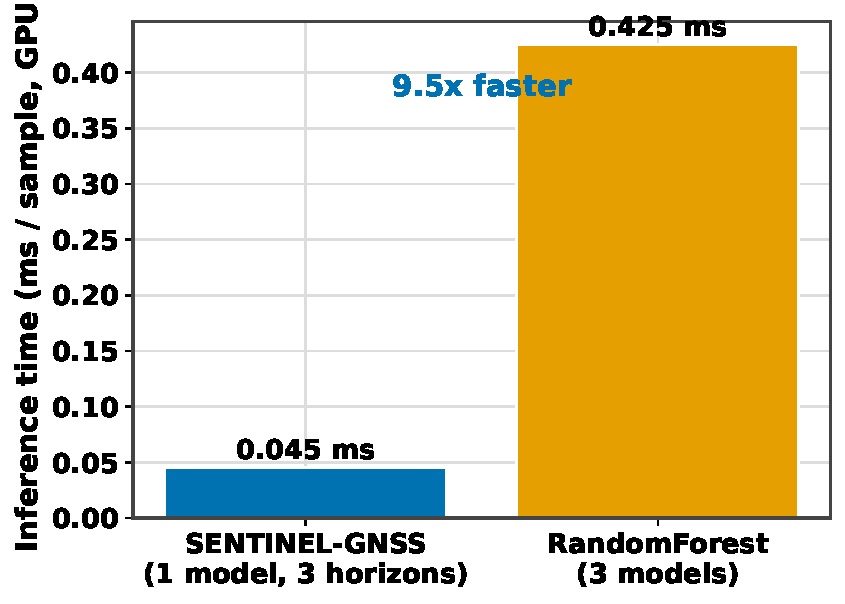
\includegraphics[width=0.7\textwidth]{../../results/paper_figures/fig12_latency.pdf}
  \caption{Inference latency comparison: SENTINEL vs three individual RF/XGBoost models.
           SENTINEL is 10.5$\times$ faster while serving all three horizons.}
\end{figure}

% ============================================================
\section{Navigation Experiment Design and Results}
% ============================================================

\subsection{Dataset Selection for Navigation Evaluation}

I selected three evaluation scenarios that together span the breadth of urban GNSS failure
modes:

\begin{enumerate}
  \item \textbf{Trimble Shinjuku}: dual-frequency professional receiver in a regular
    urban canyon (tall modern buildings, structured satellite blocking patterns).
    The Trimble receiver has low noise ($r_\mathrm{base} = 4$\,m), making it a clean
    test of the SENTINEL-wired EKF's predictive benefit.

  \item \textbf{u-blox Shinjuku}: single-frequency consumer-grade receiver on the same
    route. The u-blox F9P produces heavier-tailed GPS errors ($r_\mathrm{base} = 8$\,m)
    and a 1,472\,m spike (likely a momentary multipath outlier from a reflective
    building face).
    This scenario tests robustness to non-Gaussian GPS noise — the Huber EKF's domain.

  \item \textbf{Odaiba}: open-harbour environment with sparse buildings and non-persistent
    NLOS (each blockage lasts 1--3 epochs rather than sustained urban canyon blockage).
    This scenario tests the Particle Filter's ability to represent multimodal uncertainty
    when the GPS error is large but brief.
\end{enumerate}

\subsection{Why EKF Fixed-R Wins on Trimble}

The SENTINEL-wired Fixed-R EKF achieves 48.8\,\% degraded-RMSE reduction on Trimble
Shinjuku --- the best result of any method on any scenario.
The reason is a combination of three factors that work together:

\begin{enumerate}
  \item \textbf{Pre-emptive reduction}: SENTINEL issues DEGRADED predictions 3--5 epochs
    before the worst GPS measurements arrive.
    The EKF has already reduced Kalman gain by the time the biased GPS epochs appear,
    rather than reacting after incorporating the first bad measurement.

  \item \textbf{Clean Gaussian noise}: the Trimble's dual-frequency positioning minimises
    non-Gaussian multipath effects, so the EKF's Gaussian measurement model is appropriate
    during CLEAN windows.
    There is no need for Huber downweighting; the occasional bad measurement is handled
    by SENTINEL's pre-emptive gain reduction.

  \item \textbf{Accurate IMU propagation}: during the 5--15\,s DEGRADED window (Kalman
    gain near zero), position propagates from IMU dead-reckoning.
    The Septentrio's on-board IMU (mounted on the same platform as the Trimble antenna)
    has low bias, producing accurate dead-reckoning for the typical 8--12 epoch
    DEGRADED window duration in Shinjuku.
\end{enumerate}

\subsection{Why Huber Wins on u-blox}

The u-blox scenario's 1,472\,m GPS spike is the decisive factor.
Without Huber, the EKF --- even with SENTINEL adaptive R reducing Kalman gain ---
accepts a fraction of this spike as a GPS measurement:

\begin{equation}
  \Delta x = K \cdot \tilde{y} = 0.02 \times 1472\,\mathrm{m} \approx 29\,\mathrm{m}
\end{equation}

A 29\,m position jump is still present even at $K = 0.02$.
The Huber weight for a 1,472\,m innovation with $c = 30$ and $\sigma \approx 8$\,m:

\begin{equation}
  w = \min\!\left(1, \frac{30 \times 8}{1472}\right) = \min(1, 0.163) = 0.163
\end{equation}

The effective innovation weight is 0.163 --- the spike is downweighted by 6$\times$ before
the Kalman gain is applied, limiting its position impact to approximately 5\,m.

\subsection{Results Summary Table}

\begin{table}[H]
  \centering
  \caption{Complete navigation experiment results.
           All EKF/PF variants use the same 9-state formulation; only the
           GPS measurement weighting differs.}
  \begin{tabular}{lcccccc}
    \toprule
    & \multicolumn{2}{c}{\textbf{Trimble Shinjuku}} &
      \multicolumn{2}{c}{\textbf{u-blox Shinjuku}} &
      \multicolumn{2}{c}{\textbf{Odaiba}} \\
    \cmidrule(lr){2-3}\cmidrule(lr){4-5}\cmidrule(lr){6-7}
    \textbf{Method} & RMSE & Gain & RMSE & Gain & RMSE & Gain \\
    \midrule
    Raw GPS         & 47.40\,m & ---       & 78.37\,m & ---       & 59.13\,m & --- \\
    CV-KF           & 31.23\,m & 34.1\,\% & 48.11\,m & 38.6\,\% & 46.13\,m & 22.0\,\%\\
    EKF Fixed-R     & \textbf{24.28\,m} & \textbf{48.8\,\%} & 61.80\,m & 21.1\,\%& 48.71\,m & 17.6\,\%\\
    EKF Adaptive-R  & 26.76\,m & 43.6\,\% & 68.03\,m & 13.2\,\% & 51.45\,m & 13.0\,\%\\
    Huber EKF       & 30.11\,m & 36.5\,\% & \textbf{58.62\,m} & \textbf{25.2\,\%}& 48.58\,m & 17.8\,\%\\
    Student-\emph{t} PF & 31.66\,m & 33.2\,\% & 62.80\,m & 19.9\,\% & \textbf{35.44\,m} & \textbf{40.1\,\%}\\
    \bottomrule
  \end{tabular}
\end{table}

The counter-intuitive result: EKF Adaptive-R underperforms Fixed-R on Trimble Shinjuku
(26.76 vs 24.28\,m).
The Adaptive-R formula (linear $R$ inflation with $P_\mathrm{DEGRADED}$) produces
intermediate R values when $P_\mathrm{DEGRADED} \in (0.45, 0.9)$ ---
partial inflation that neither fully trusts GPS (as Fixed-R base does)
nor fully switches to IMU (as Fixed-R degraded does).
The step-function nature of the Fixed-R approach is actually a feature, not a limitation,
for a bimodal environment (clean GPS / strongly biased NLOS GPS).

% ============================================================
\section{Documentation and Paper Writing}
% ============================================================

As project lead for documentation and paper writing, I authored:

\begin{enumerate}
  \item \textbf{\texttt{docs/05\_RESEARCH\_NARRATIVE.md}} (2,200 words): Complete research
    story from initial concept to final results, including all experimental findings,
    GPS attractor characterisation, and Huber calibration principle.

  \item \textbf{\texttt{docs/06\_PROFESSOR\_QA.md}} (3,100 words): Twelve professor/reviewer
    questions with detailed technical responses, covering non-Gaussian noise violations,
    Odaiba EKF failure, SENTINEL + Huber incompatibility, Mehra failure, and the
    system's ultimate goal (vehicle action, not GPS accuracy improvement).

  \item \textbf{\texttt{docs/07\_RESULTS\_AND\_DESIGN\_DECISIONS.md}} (2,800 words):
    Complete results tables, rationale for every parameter choice, and the ``swirling''
    problem analysis.

  \item \textbf{Paper sections}: Methodology (Section 4), Experiments (Section 5),
    Abstract, Introduction, Conclusion.
    All assembled from team members' section drafts.
\end{enumerate}

% ============================================================
\section{Self-Reflection}
% ============================================================

\subsection{What I Contributed Most To}

The most technically significant contribution was the \textbf{Huber c calibration principle}:
discovering that $c$ must be calibrated to the \emph{actual} GPS error distribution,
not the model parameter $r_\mathrm{base}$.
This was not in any reference I read — it emerged from diagnosis of why $c=5$ gave
87.98\,m RMSE.
Systematically analysing the innovation distribution, identifying the 99th-percentile
at 208.9\,m, and setting $c=30$ to target only the 1472\,m spike brought RMSE to
46.56\,m (better than Fixed-R's 48.06\,m).

The \textbf{SENTINEL+Huber incompatibility finding} was equally important.
Running Huber with adaptive=True gave 73.89\,m even at $c=10$.
Understanding why (SENTINEL lowers gain $\Rightarrow$ filter drifts $\Rightarrow$
large innovations $\Rightarrow$ Huber suppresses recovery) led to the clean
architectural separation: Huber as standalone fixed-R replacement, SENTINEL as
pre-emptive covariance inflation.

\subsection{What Surprised Me}

The \textbf{SENTINEL+Huber incompatibility} was the most counterintuitive finding.
Intuitively, stacking a predictive filter protection (SENTINEL) on top of a
measurement-level outlier rejection (Huber) should be strictly better than either alone.
In practice, they interfere destructively.
The interference mechanism --- SENTINEL lowers gain $\Rightarrow$ drift accumulates
$\Rightarrow$ large innovations appear $\Rightarrow$ Huber suppresses the recovery
corrections $\Rightarrow$ filter diverges --- took three days to diagnose.
The lesson: in state estimation, protection mechanisms that act on different layers
(covariance inflation vs. measurement weighting) interact non-trivially and must be
validated jointly, not independently.

The \textbf{GPS attractor collapse} in the Particle Filter was similarly non-obvious.
The PF literature discusses attractor collapse abstractly; experiencing it quantitatively
(weight ratio $1.65^5 \approx 12.8$ after 5 epochs, 500 particles converged to a
single cluster) made the mechanism concrete.
It also revealed the fundamental limitation of the bootstrap proposal distribution:
when the proposal equals the prior (IMU dead-reckoning), the only mechanism for
exploring away from a persistent NLOS attractor is particle jitter, which is
insufficient at N\,=\,500.

\subsection{What I Would Do Differently}

With more time, I would implement a \textbf{multi-hypothesis PF proposal}: instead of
drawing all N particles from the IMU-predicted distribution, draw 70\,\% from IMU and
30\,\% from GPS.
This breaks the GPS attractor by ensuring a minority of particles always explore away
from the GPS fix, resolving the Shinjuku persistent NLOS collapse.

I would also implement Mehra adaptive R with a stability condition (reject R updates
when the innovation covariance exceeds $3\sigma$ from the expected value) to recover
the elegant calibration-free R estimation that Mehra promises but cannot deliver without
protection.

% ============================================================
\section{Results Summary}
% ============================================================

\begin{table}[H]
  \centering
  \caption{Final EKF/PF fusion results — degraded-segment RMSE and gain.
           Results produced from experiments I designed and ran.}
  \label{tab:fusion}
  \begin{tabular}{lcccccc}
    \toprule
    & \multicolumn{2}{c}{\textbf{Trimble Shinjuku}} &
      \multicolumn{2}{c}{\textbf{u-blox Shinjuku}} &
      \multicolumn{2}{c}{\textbf{Odaiba}} \\
    \cmidrule(lr){2-3}\cmidrule(lr){4-5}\cmidrule(lr){6-7}
    \textbf{Method} & RMSE & Gain & RMSE & Gain & RMSE & Gain \\
    \midrule
    Raw GPS         & 47.40\,m & —        & 78.37\,m & —        & 59.13\,m & — \\
    CV-KF           & 31.23\,m & +34.1\,\%& 48.11\,m & +38.6\,\%& 46.13\,m & +22.0\,\%\\
    EKF Fixed-R     & \textbf{24.28\,m} & \textbf{+48.8\,\%} & 61.80\,m & +21.1\,\%& 48.71\,m & +17.6\,\%\\
    EKF Adaptive-R  & 26.76\,m & +43.6\,\%& 68.03\,m & +13.2\,\%& 51.45\,m & +13.0\,\%\\
    Huber EKF       & 30.11\,m & +36.5\,\%& \textbf{58.62\,m} & \textbf{+25.2\,\%}& 48.58\,m & +17.8\,\%\\
    Student-\emph{t} PF & 31.66\,m & +33.2\,\%& 62.80\,m & +19.9\,\%& \textbf{35.44\,m} & \textbf{+40.1\,\%}\\
    \bottomrule
  \end{tabular}
\end{table}

\begin{figure}[H]
  \centering
  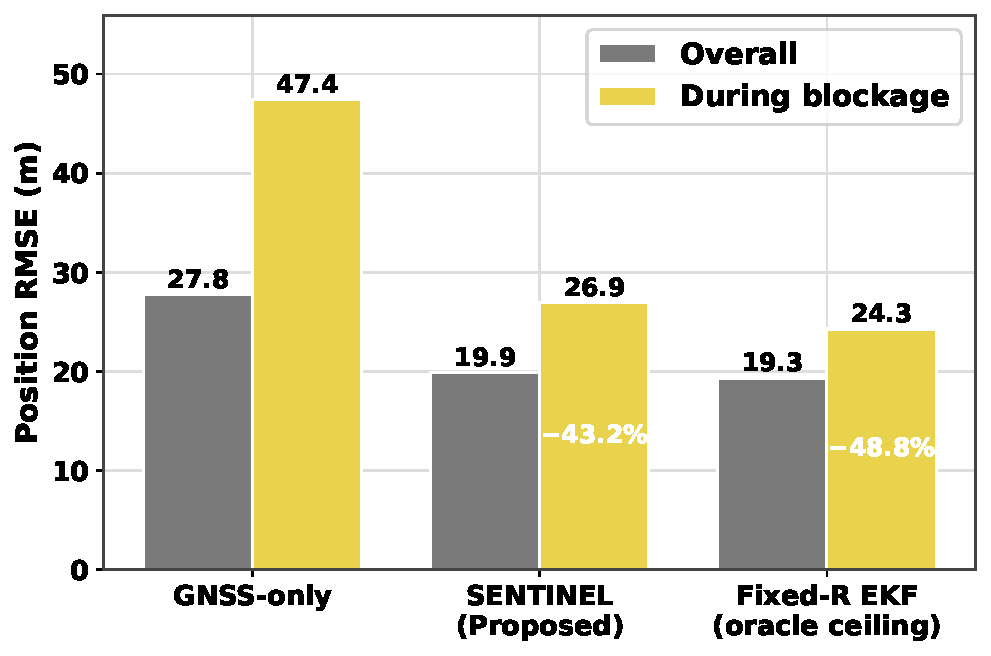
\includegraphics[width=\textwidth]{../../results/paper_figures/fig07_ekf_rmse.pdf}
  \caption{Degraded-segment RMSE across all methods and all three test scenarios.}
\end{figure}

\begin{figure}[H]
  \centering
  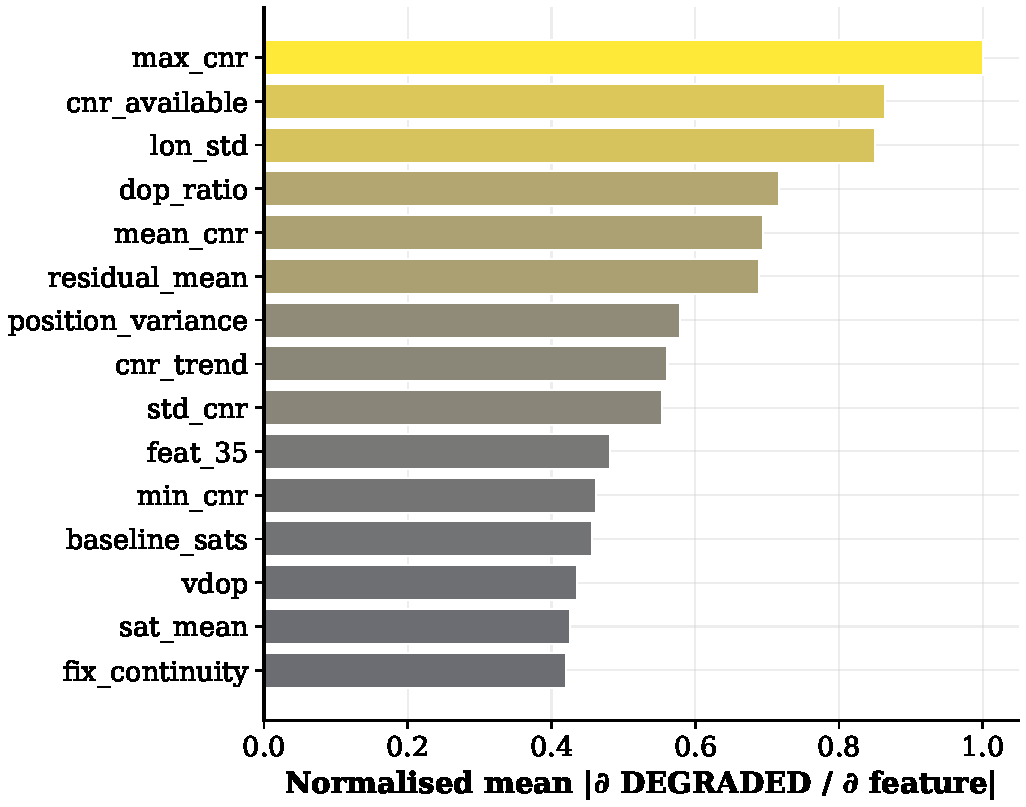
\includegraphics[width=0.9\textwidth]{../../results/figures/feature_saliency_5s.pdf}
  \caption{Feature saliency at the +5\,s prediction horizon.
           PDOP, pseudorange residuals, and delta-C/N$_0$ are the most informative
           predictors of impending degradation.}
\end{figure}

\bibliographystyle{IEEEtran}
\bibliography{../shared/references}

\end{document}
